\hypertarget{roadmap}{%
\subsection{Roadmap}\label{roadmap}}

\hypertarget{motivation}{%
\subsubsection{Motivation}\label{motivation}}

This pattern shows how your group can define the scope of their project
and make a realistic plan to address it. This pattern provides the
backbone of our pattern language. It can be used to find a shared goal.

\hypertarget{context}{%
\subsubsection{Context}\label{context}}

\href{http://peeragogy.github.io/pattern-peeragogy.html}{Peeragogy} has
both distributed and centralized aspects. The discussants or
contributors who collaborate on a project have different points of view
and heterogeneous priorities, but they come together in conversations
and joint activities.

\hypertarget{forces}{%
\subsubsection{Forces}\label{forces}}

\begin{quote}

\includegraphics{images/variety.png} \textbf{Variety}: people have
different goals and interests in mind.\\

\includegraphics{images/clarity.png} \textbf{Clarity}: some goals may be
quite specific, and some rather vague.\\

\includegraphics{images/coherence.png} \textbf{Coherence}: only some of
these goals will be well-aligned.
\end{quote}

\hypertarget{problem}{%
\subsubsection{Problem}\label{problem}}

In order to collaborate, people need a way to share current, though
incomplete, understanding of the space they are working in, and to
nurture relationships with one another and the other elements of this
space. At the outset, there may not even be a coherent vision for a
project -- but a only loose collection of motivations and sentiments.
Once the project is up and running, people are likely to pull in
different directions.

\hypertarget{solution}{%
\subsubsection{Solution}\label{solution}}

Building a guide to the goals, activities, experiments and working
methods can help {{Newcomers}} and old-timers alike understand their
relationship with the project. It may combine features of a manifesto, a
syllabus, and an issue tracker. It may be a design pattern or a pattern
language {{[}3{]}}. The distinguishing qualities of a project Roadmap
are that it should be adaptive to circumstances, and that it should
ultimately get us from \emph{here} to \emph{there}. By this same token,
any given version of the roadmap is seen as fallible. In lieu of
widespread participation, the project's {{Wrapper}} should attempt to
synthesize an accurate roadmap that is informed by participants'
behavior, and should help moderate in case of conflict. Nevertheless,
full consensus is not necessary: different goals, with different
\emph{heres} and \emph{theres}, can be pursued separately, while
maintaining communication.

\hypertarget{rationale}{%
\subsubsection{Rationale}\label{rationale}}

The group evolves from a less-sophisticated to a more-sophisticated
manner of operating by using the roadmap. Using the roadmap builds a
collective awareness of how things are working in practice. In the
Peeragogy project our initial roadmap was a ``crowdsourced'' outline of
the first edition of the \emph{Peeragogy Handbook}. Later, it took the
form of a schedule of meetings following a regular {{Heartbeat}},
supplemented by a list of upcoming deadlines. Most recently, our roadmap
is expressed in the emergent objectives collected at the end of current
paper. We have seen that a list of nice-to-have features created in a
top-down fashion is comparatively unlikely to go anywhere! A backlog of
tasks and a realistic plan for accomplishing them are vastly different
things. An adaptive roadmap is an antidote to {{Tunnel Vision}}
{{[}1{]}}.

\hypertarget{resolution}{%
\subsubsection{Resolution}\label{resolution}}

An emergent roadmap is rooted in real problems and justifiable
solutions-in-progress in all their \textbf{variety} and communicates
both resolution and follow-through. The process of meshing varied issues
with one another requires thought and discussion, and this encourages
\textbf{clarity}. The test of \textbf{coherence} is that contributed
goals and ideas should be actionable. The ultimate quality-control test
is if it worked, i.e., did it come to pass that the task(s) the roadmap
was created to achieve ended up being achieved? If all of the issues
that the roadmap outlines are not resolved, the roadmap itself should be
revised. Without a roadmap, we would never know.

\hypertarget{example-1}{%
\subsubsection{Example 1}\label{example-1}}

The \emph{Help} link present on every Wikipedia page could be seen as a
localized {{Roadmap}} for individual user engagement: it tells users
what they can do with the site, and gives instructions on how to do
it.\footnote{\url{https://en.wikipedia.org/wiki/Help:Contents}} someone
who knows what they're doing, there are around 30 pages listing articles
with various kinds of problems, for example articles tagged with style
issues, or ``orphaned'' articles (i.e., articles with no links from
other pages in the encyclopedia).\footnote{\url{https://en.wikipedia.org/wiki/Category:Wikipedia_article_cleanup}},\footnote{\url{https://en.wikipedia.org/wiki/Category:Wikipedia_articles_with_style_issues}},\footnote{\url{https://en.wikipedia.org/wiki/Category:All_orphaned_articles}}
In 2010-2011, Wikimedia developed a strategic plan drawing on community
input {{[}2{]}}. In 2015, a two-week Community Consultation was carried
out; synthesis resulted in ``a direction that will guide the decisions
for the organization.''\footnote{\url{https://blog.wikimedia.org/2015/02/23/strategy-consultation/}}
Community-organized WikiProjects often invite and guide involvement on
{{A specific project}}.

\hypertarget{example-2}{%
\subsubsection{Example 2}\label{example-2}}

In a future university run in a peer produced manner, a fancy
President's Residence presumably wouldn't be needed. Leadership would be
carried out in a more collaborative and distributed fashion. However,
depending on just how distributed things are, it may turn out to be
useful for project facilitators to gather at a University Hall. Whereas
there is strength in numbers, there is leverage in organization. This is
what the {{Roadmap}} provides.

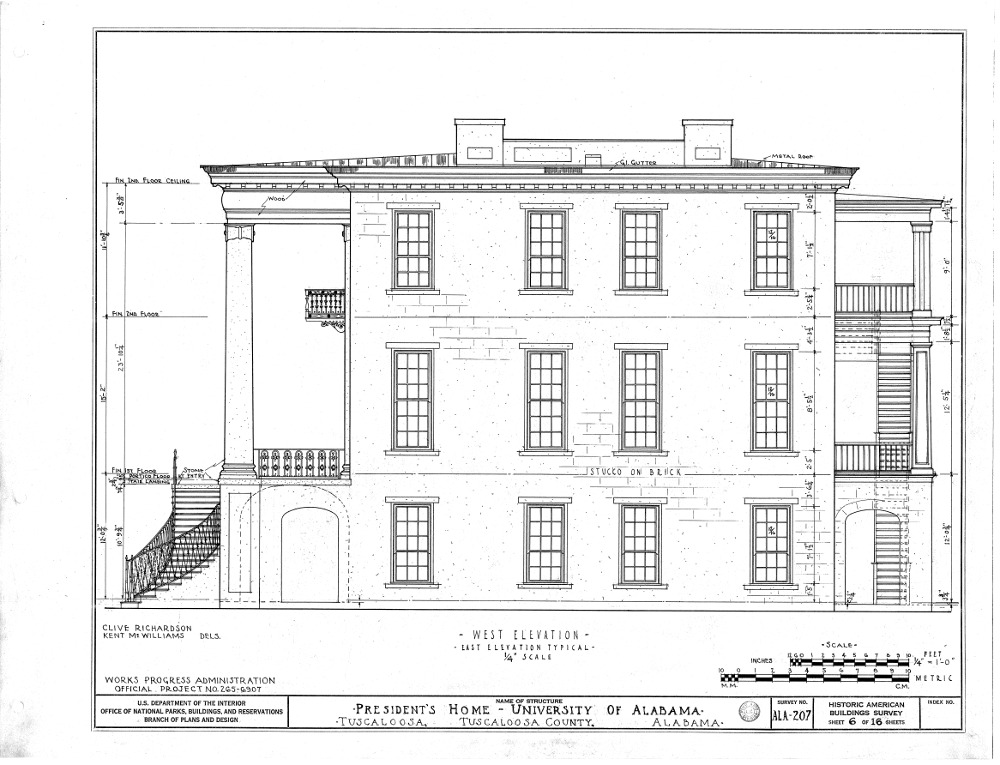
\includegraphics{images/alabama-small.jpg}\\
\emph{President's Residence, University of Alabama.}

\hypertarget{whats-next-in-the-peeragogy-project}{%
\subsubsection{What's Next in the Peeragogy
Project}\label{whats-next-in-the-peeragogy-project}}

If it becomes clear that something needs to change about the project,
that is a clue that we might need to revise our patterns or record a new
one. We can use the names of the patterns to tag our upcoming tasks.

\hypertarget{references}{%
\subsubsection{References}\label{references}}

\begin{enumerate}
\def\labelenumi{\arabic{enumi}.}
\item
  David M. Dikel, David Kane, and James R. Wilson. 2001. \emph{Software
  architecture: Organizational principles and patterns}. Pearson
  Education.
\item
  Eugene Eric Kim and others. 2011. \emph{Wikimedia Strategic Plan: A
  collaborative vision for the movement through 2015}. Wikimedia
  Foundation.
\item
  Christian Kohls. 2010. The structure of patterns. \emph{Proceedings of
  the 17th Conference on Pattern Languages of Programs}, ACM, 12.
\end{enumerate}

\begin{center}\rule{0.5\linewidth}{0.5pt}\end{center}
